\begin{figure}[htbp]
			\centering
			\begin{tikzpicture}[scale=0.95,>=latex,
				trave/.style={line width=1.2pt},
				forza/.style={black, line width=1pt},
				quota/.style={black, line width=0.4pt},
				diagN/.style={black, line width=0.8pt},
				diagT/.style={black, line width=0.8pt},
				diagM/.style={black, line width=0.8pt},
				hatch/.style={gray!40, line width=0.3pt},
				]
				% ── Parametri vincoli (convenzione C06/C07) ──
				\def\tw{0.15}\def\thR{0.28}\def\rn{0.06}
				\def\rw{0.05}\def\bw{0.09}\def\gw{0.22}\def\hh{0.10}
				\def\Lb{4}        % lunghezza trave (unità di disegno)
				\def\hT{0.5}      % altezza visiva di P/2 (diagrammi N, T)
				\def\hM{0.8}      % profondità visiva di Pl/4 (diagramma M)
				% ── trave + cerniera A + carrello inclinato B + perni + etichette ──
				\def\supporti{%
					\draw[trave] (0,0) -- (\Lb,0);
					\draw[thick] (0,0) -- (-\tw,-\thR) -- (\tw,-\thR) -- cycle;
					\draw[thick] (-\gw,-\thR) -- (\gw,-\thR);
					\foreach \x in {-0.16,-0.08,0,0.08,0.16}
					\draw[thin] (\x,-\thR) -- ++(-0.07,-\hh);
					\begin{scope}[shift={(\Lb,0)}, rotate=45]
						\draw[thick] (0,0) -- (-\tw,-\thR) -- (\tw,-\thR) -- cycle;
						\draw[thick] (-\bw,-\thR-\rw-0.01) circle (\rw);
						\draw[thick] (\bw,-\thR-\rw-0.01) circle (\rw);
						\draw[thick] (-\gw,-\thR-2*\rw-0.04) -- (\gw,-\thR-2*\rw-0.04);
						\foreach \x in {-0.16,-0.08,0,0.08,0.16}
						\draw[thin] (\x,-\thR-2*\rw-0.04) -- ++(-0.07,-\hh);
					\end{scope}
					\draw[thick, fill=white] (0,0) circle (\rn);
					\draw[thick, fill=white] (\Lb,0) circle (\rn);
					\node[above left=-2pt, font=\small] at (0,0) {$A$};
					\node[above, font=\small] at (\Lb,0) {$B$};}
				
				% ========================= (a) schema =========================
				\begin{scope}[xshift=0cm, yshift=0cm]
					\supporti
					\draw[thin, gray!60] (\Lb,0) -- ++(0:0.95);   % prolungamento asse trave (riferimento orizzontale)
					\draw[thin, gray!60] (\Lb,0) -- ++(45:0.95);  % direzione del piano di scorrimento
					\draw[gray!60] (\Lb+0.62,0) arc (0:45:0.62);
					\node[gray!80, font=\scriptsize] at (\Lb+0.86,0.30) {$\pi/4$};
					\draw[->, forza] (\Lb/2, 0.95) -- (\Lb/2, 0.03);
					\node[right, font=\small] at (\Lb/2+0.04, 0.58) {$P$};
					\node[below, font=\footnotesize] at (\Lb/2,-0.02) {$C$};
					\def\yq{-0.80}
					\draw[quota, <->] (0,\yq) -- (\Lb/2,\yq);
					\draw[quota] (0,\yq+0.10) -- (0,\yq-0.10);
					\draw[quota] (\Lb/2,\yq+0.10) -- (\Lb/2,\yq-0.10);
					\node[above, font=\footnotesize] at (\Lb/4,\yq) {$\ell/2$};
					\node[font=\small] at (2*\Lb/3,-1.0) {(a)};
				\end{scope}
				
				% ============ (b) N: uniforme in compressione, sotto l'asse ============
				\begin{scope}[xshift=6.8cm, yshift=0cm]
					\foreach \x in {0.10,0.30,...,3.90}\draw[hatch] (\x,0)--(\x,-\hT);
					\draw[diagN] (0,0)--(0,-\hT)--(\Lb,-\hT)--(\Lb,0);
					\node[font=\small] at (\Lb/2,-0.5*\hT) {$\boldsymbol{\ominus}$};
					\node[left, font=\small] at (0,-\hT-0.2) {$\tfrac{P}{2}$};
					\supporti
					\node[font=\small] at (2*\Lb/3,-1.0) {(b)};
				\end{scope}
				
				% ========== (c) T: +P/2 sopra (AC), -P/2 sotto (CB) ==========
				\begin{scope}[xshift=0cm, yshift=-2.25cm]
					\foreach \x in {0.10,0.30,...,1.90}\draw[hatch] (\x,0)--(\x,\hT);
					\foreach \x in {2.10,2.30,...,3.90}\draw[hatch] (\x,0)--(\x,-\hT);
					\draw[diagT] (0,0)--(0,\hT)--(\Lb/2,\hT)--(\Lb/2,-\hT)--(\Lb,-\hT)--(\Lb,0);
					\node[font=\small] at (\Lb/4,0.5*\hT) {$\boldsymbol{\oplus}$};
					\node[font=\small] at (3*\Lb/4,-0.5*\hT) {$\boldsymbol{\ominus}$};
					\node[right, font=\small] at (\Lb/2,\hT) {$\tfrac{P}{2}$};
					\node[left, font=\small] at (\Lb/2,-\hT) {$\tfrac{P}{2}$};
					\supporti
					\node[font=\small] at (2*\Lb/3,-1.0) {(c)};
				\end{scope}
				
				% ============= (d) M: triangolo sotto, max in C =============
				\begin{scope}[xshift=6.8cm, yshift=-2.25cm]
					\foreach \x in {0.20,0.40,...,1.80}{%
						\pgfmathsetmacro{\h}{-\hM*\x/(\Lb/2)}\draw[hatch] (\x,0)--(\x,\h);}
					\foreach \x in {2.20,2.40,...,3.80}{%
						\pgfmathsetmacro{\h}{-\hM*(\Lb-\x)/(\Lb/2)}\draw[hatch] (\x,0)--(\x,\h);}
					\draw[diagM] (0,0)--(\Lb/2,-\hM)--(\Lb,0);
					\node[above, font=\small] at (\Lb/2,-\hM-0.02) {$\tfrac{P\ell}{4}$};
					\supporti
					\node[font=\small] at (2*\Lb/3,-1.0) {(d)};
				\end{scope}
				
			\end{tikzpicture}
			\caption{Trave con cerniera in $A$ e carrello inclinato di $\pi/4$
				in $B$, con forza concentrata $P$ in mezzeria $C$:
				(a)~schema strutturale; (b)~sforzo normale $N$, uniforme in
				compressione $-P/2$; (c)~taglio $T$, pari a $+P/2$ nel tratto
				$AC$ e $-P/2$ nel tratto $CB$, con salto $-P$ in $C$;
				(d)~momento flettente $M$, lineare a tratti con massimo
				$P\ell/4$ in $C$.}
			\label{fig:stat_misto_iso_01}
		\end{figure}
